% Architecture diagram for Morphon — standalone TikZ figure
% Compiled into PDF by the Makefile.
\documentclass[tikz,border=4pt]{standalone}
\usepackage{tikz}
\usetikzlibrary{positioning,arrows.meta,fit,backgrounds,shadows.blur,calc}

\definecolor{fastclr}{HTML}{5b9bd5}
\definecolor{medclr}{HTML}{70ad47}
\definecolor{slowclr}{HTML}{ed7d31}
\definecolor{glaclr}{HTML}{a5a5a5}
\definecolor{endoclr}{HTML}{c00000}
\definecolor{ioclr}{HTML}{7030a0}

\begin{document}
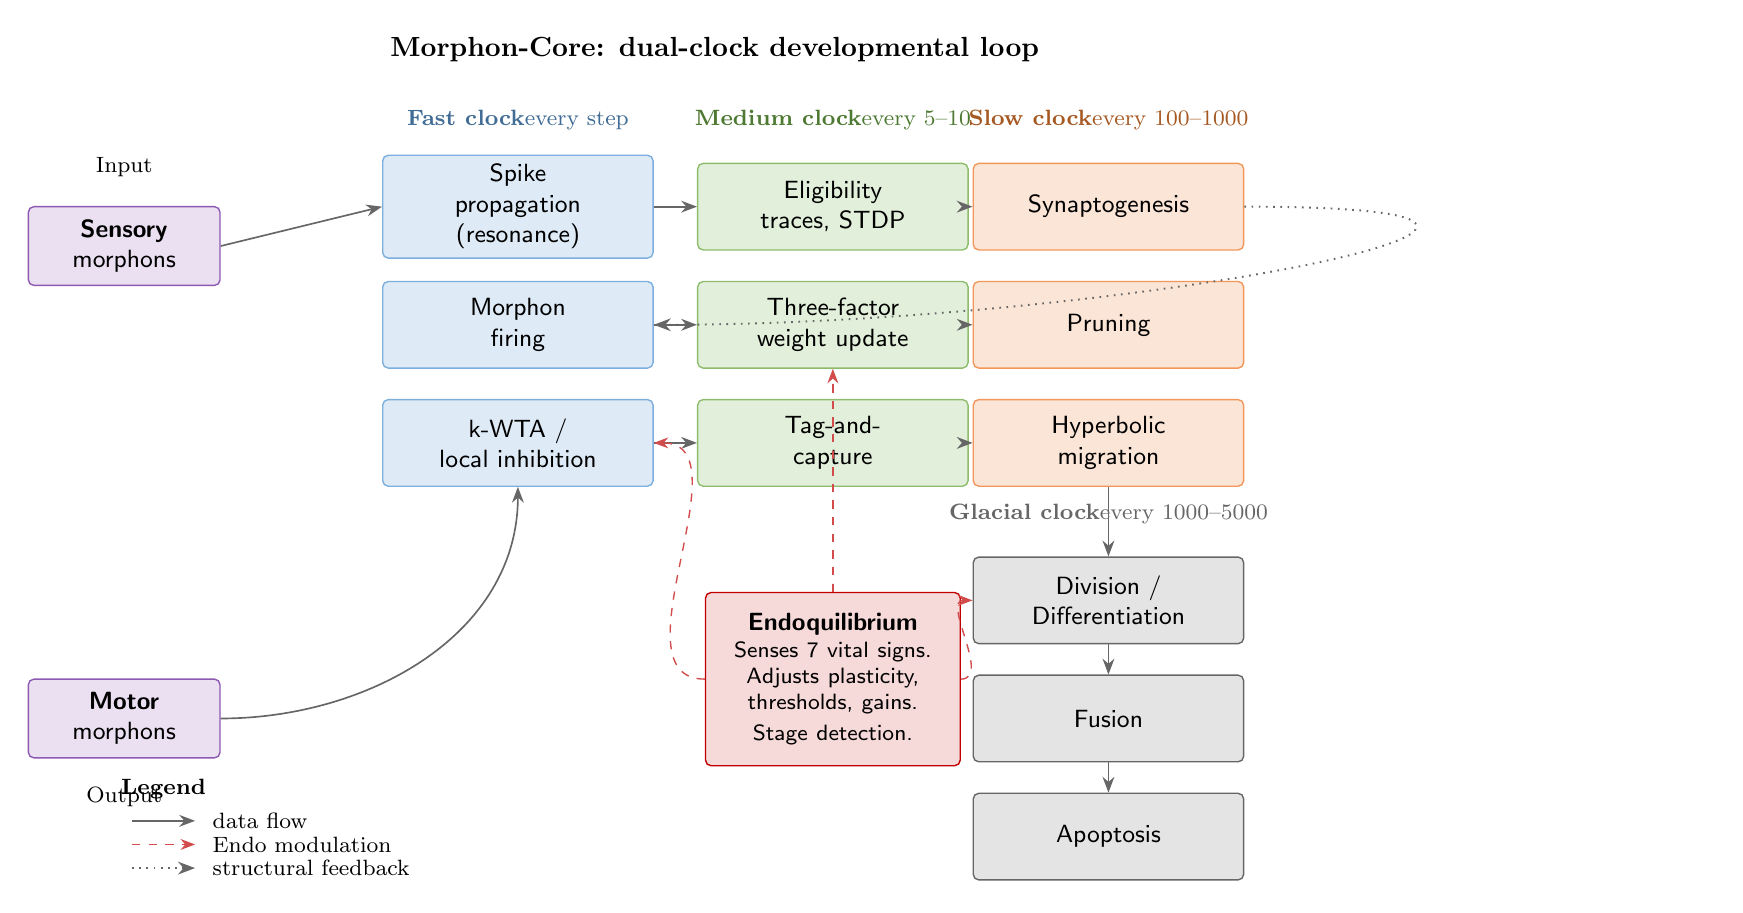
\begin{tikzpicture}[
  font=\sffamily\small,
  node distance=4mm and 6mm,
  box/.style={
    rectangle, rounded corners=2pt, draw=black, line width=0.5pt,
    text width=32mm, align=center, minimum height=11mm, fill=white,
  },
  fast/.style={box, fill=fastclr!20, draw=fastclr!80},
  med/.style={box, fill=medclr!20, draw=medclr!80},
  slow/.style={box, fill=slowclr!20, draw=slowclr!80},
  glac/.style={box, fill=glaclr!30, draw=black!60},
  endo/.style={box, fill=endoclr!15, draw=endoclr, text width=30mm, minimum height=22mm},
  io/.style={box, fill=ioclr!15, draw=ioclr!80, text width=22mm, minimum height=10mm},
  arrow/.style={-Stealth, line width=0.6pt, draw=black!60},
  modarrow/.style={-Stealth, line width=0.5pt, draw=endoclr!70, dashed},
]

% Title
\node (title) at (0, 6.5) [font=\bfseries] {Morphon-Core: dual-clock developmental loop};

% Input column
\node[io] (sensory) at (-7.5, 4.0) {\textbf{Sensory}\\morphons};
\node[io] (motor)   at (-7.5, -2.0) {\textbf{Motor}\\morphons};
\node[font=\footnotesize, text width=20mm, align=center] at (-7.5, 5.0) {Input};
\node[font=\footnotesize, text width=20mm, align=center] at (-7.5, -3.0) {Output};

% Fast path
\node[fast] (fast1) at (-2.5, 4.5) {Spike\\propagation\\(resonance)};
\node[fast] (fast2) at (-2.5, 3.0) {Morphon\\firing};
\node[fast] (fast3) at (-2.5, 1.5) {k-WTA /\\local inhibition};

% Medium path
\node[med] (med1) at ( 1.5, 4.5) {Eligibility\\traces, STDP};
\node[med] (med2) at ( 1.5, 3.0) {Three-factor\\weight update};
\node[med] (med3) at ( 1.5, 1.5) {Tag-and-\\capture};

% Slow path
\node[slow] (slow1) at ( 5.0, 4.5) {Synaptogenesis};
\node[slow] (slow2) at ( 5.0, 3.0) {Pruning};
\node[slow] (slow3) at ( 5.0, 1.5) {Hyperbolic\\migration};

% Glacial path
\node[glac] (glac1) at ( 5.0, -0.5) {Division /\\Differentiation};
\node[glac] (glac2) at ( 5.0, -2.0) {Fusion};
\node[glac] (glac3) at ( 5.0, -3.5) {Apoptosis};

% Endoquilibrium
\node[endo] (endo) at (1.5, -1.5) {\textbf{Endoquilibrium}\\\footnotesize Senses 7 vital signs.\\Adjusts plasticity,\\thresholds, gains.\\Stage detection.};

% Period labels
\node[font=\bfseries\footnotesize, fastclr!70!black] at (-2.5, 5.6) {Fast clock\\\textmd{every step}};
\node[font=\bfseries\footnotesize, medclr!70!black]  at ( 1.5, 5.6) {Medium clock\\\textmd{every 5--10}};
\node[font=\bfseries\footnotesize, slowclr!70!black] at ( 5.0, 5.6) {Slow clock\\\textmd{every 100--1000}};
\node[font=\bfseries\footnotesize, black!60]         at ( 5.0, 0.6) {Glacial clock\\\textmd{every 1000--5000}};

% Arrows: I/O to fast
\draw[arrow] (sensory.east) -- (fast1.west);
\draw[arrow] (motor.east) to[out=0,in=270] (fast3.south);

% Fast → Medium → Slow chain
\draw[arrow] (fast1.east) -- (med1.west);
\draw[arrow] (fast2.east) -- (med2.west);
\draw[arrow] (fast3.east) -- (med3.west);
\draw[arrow] (med1.east) -- (slow1.west);
\draw[arrow] (med2.east) -- (slow2.west);
\draw[arrow] (med3.east) -- (slow3.west);

% Slow → Glacial
\draw[arrow] (slow3.south) -- (glac1.north);
\draw[arrow] (glac1.south) -- (glac2.north);
\draw[arrow] (glac2.south) -- (glac3.north);

% Endoquilibrium influence (dashed)
\draw[modarrow] (endo.north) to[out=90,in=270] (med2.south);
\draw[modarrow] (endo.east) to[out=0,in=180] (glac1.west);
\draw[modarrow] (endo.west) to[out=180,in=0] (fast3.east);

% Recurrent feedback loop
\draw[arrow, dotted, line width=0.7pt] (slow1.east) to[out=0,in=0,looseness=2] (fast2.east);

% Legend
\begin{scope}[shift={(-7.0, -3.5)}]
  \node[font=\footnotesize\bfseries] at (0, 0.6) {Legend};
  \draw[arrow] (-0.4, 0.2) -- (0.4, 0.2);
  \node[font=\footnotesize, anchor=west] at (0.5, 0.2) {data flow};
  \draw[modarrow] (-0.4, -0.1) -- (0.4, -0.1);
  \node[font=\footnotesize, anchor=west] at (0.5, -0.1) {Endo modulation};
  \draw[arrow, dotted, line width=0.7pt] (-0.4, -0.4) -- (0.4, -0.4);
  \node[font=\footnotesize, anchor=west] at (0.5, -0.4) {structural feedback};
\end{scope}

\end{tikzpicture}
\end{document}
